\documentclass[a4paper,10pt]{article}
\usepackage[utf8]{inputenc}
\usepackage[MeX]{polski}
\usepackage{tikz}
\usepackage{fancyvrb}

\title{Grafy i Sieci. Sprawozdanie 2. \\ \small{SK11 Kolorowanie grafu za pomocą przeszukiwania z tabu.}}
\author{Michał Aniserowicz, Jakub Turek}
\date{}

\begin{document}

\maketitle

\section{Temat projektu}

SK11 Kolorowanie grafu za pomocą przeszukiwania z tabu.

\section{Opis algorytmu}
Zadaniem programu jest pokolorowanie wierzchołków zadanego grafu z użyciem jak najmniejszej liczby kolorów.
Kolorowanie odbywa się z wykorzystaniem heurystycznego algorytmu przeszukiwania z tabu.
Węzłem przestrzeni przeszukiwań jest pokolorowany (legalnie bądź nie) graf.

\subsection{Sąsiedztwo}
Sąsiadami w przestrzeni przeszukiwań są takie dwa pokolorowane grafy $G$~i~$H$, że graf~$H$ można osiągnąć poprzez zmianę koloru jednego z wierzchołków grafu~$G$.

\subsection{Funkcja celu}
Algorytm dąży do minimalizacji funkcji celu\footnote{Definicja funkcji celu zaczerpnięta z: D. S. Johnson, C. R. Aragon, L. A. McGeoch, C. Schevon, Optimization by Simulated Annealing: An Experimental Evaluation; Part II, Graph Coloring and Number Partitioning, Operations Research, Vol. 39, No. 3, May-June 1991, pp. 378-406.}:

\begin{equation}
 f(G) = -\sum_{i=1}^{k} C_i^2 + \sum_{i=1}^{k} 2 C_i E_i
\end{equation}

gdzie:
\begin{itemize}
 \item $G$ - graf, dla którego liczona jest funkcja celu,
 \item $k$ - liczba kolorów użytych do pokolorowania grafu $G$,
 \item $C_i$ - liczba wierzchołków grafu $G$ pokolorowanych na $i$-ty kolor,
 \item $E_i$ - liczba krawędzi grafu $G$, których oba końce pokolorowane są na $i$-ty kolor.
\end{itemize}

Definicję funkcji należy rozumieć następująco:

\begin{enumerate}
 \item z jednej strony, faworyzowane są pokolorowania z użyciem jak najmniejszej liczby kolorów,
 \item z drugiej strony, dyskryminowane są pokolorowania nielegalne.
\end{enumerate}

\subsection{Lista tabu}
Lista tabu zawiera ograniczoną liczbę ostatnich akcji podjętych przez algorytm.
Pojedynczą akcją jest wybór wierzchołka, który zostanie pokolorowany na inny kolor.
Akcja na liście tabu jest reprezentowana przez parę \emph{identyfikator wierzchołka} oraz \emph{kolor wierzchołka przed podjęciem akcji}. 
Reprezentacja ta zapobiega badaniu jednakowych kombinacji w~kolejnych iteracjach algorytmu. Przykładowo, w~minimum lokalnym może zdarzyć się sytuacja, gdy najlepsze wartości funkcji celu będziemy osiągać poprzez cykliczną zmianę koloru tego samego wierzchołka w~kolejnych iteracjach, czego chcemy uniknąć.

\subsection{Pamięci}

W~algorytmie zostaną wykorzystane dwie pamięci:

\begin{description}
 \item [Krótkoterminowa] Realizuje listę tabu. Jej rozmiar jest parametrem algorytmu.
 \item [Długoterminowa] Przechowuje historię wszystkich akcji. Jest wykorzystywana podczas podejmowania decyzji o~wyborze najlepszej permutacji w~danej iteracji, w~momencie gdy istnieje wiele najlepszych permutacji o~jednakowej wartości funkcji celu.
\end{description}

\section{Struktury danych}
\subsection{Graf}
Podstawową strukturą danych użytą w programie jest graf, na który składa się zbiór wierchołków.
Pojednynczy wierchołek zawiera:
\begin{itemize}
 \item identyfikator wierzchołka (ciąg znaków),
 \item identyfikator przypisanego koloru (liczba całkowita),
 \item zbiór wskazań na sąsiadujące wierzchołki (kolekcja wskazań).
\end{itemize}

\subsection{Pamięć}
Pamięć to listowa struktura danych, do której kolejne wpisy dodawane są na początku listy. W~pamięci przechowywane są pary (\emph{identyfikator wierzchołka}, \emph{kolor wierzchołka}).

\begin{itemize}
 \item Pamięć długoterminowa jest realizowana poprzez przechowywanie na liście wszystkich przejść od początku działania algorytmu.
 \item Pamięć krótkoterminowa jest realizowana poprzez użycie okna o~rozmiarze $m$, umieszczonego na początku listy.
\end{itemize}

\section{Założenia programu}

\subsection{Złożoność obliczeniowa}

Złożoność obliczeniową można oszacować wyrażeniem:

\begin{equation}
	i * (nk * m + nk * n^2 + (nk * log(nk))
\end{equation}

\noindent gdzie:

\begin{itemize}
 \item $i$ - liczba iteracji,
 \item $n$ - liczba wierzchołków grafu,
 \item $m$ - rozmiar pamięci tabu.
\end{itemize}

\noindent Każda z~$i$ iteracji składa się z~następujących kroków:

\begin{enumerate}
 \item Wyznaczenie wszystkich możliwych sąsiadów aktualnego grafu, wraz ze sprawdzeniem dopuszczalności (lista tabu): $nk * m$.
 \item Obliczenie funkcji celu dla każdego dopuszczalnego sąsiada: $nk * n^2$. (Obliczenie funkcji celu wymaga odwiedzenia wszystkich wierzchołków oraz wszystkich wierzchołków z~nimi połączonych: $n^2$.)
 \item Sortowanie wyznaczonych sąsiadów ze względu na wartość funkcji celu: $nk * log(nk)$.
\end{enumerate}

\noindent Algorytm ma zatem złożoność wielomianową. 

\subsection{Dane wejściowe}

Na rysunku \ref{fig:input_data} przedstawiono przykładowe dane wejściowe. Dane wejściowe składają się z:

\begin{figure}[ht!]
	\begin{Verbatim}[frame=single]
3
A,B
C,D
A,D
C,E 
	\end{Verbatim}
	\caption{Przykładowe dane wejściowe.}
	\label{fig:input_data}
\end{figure}

\begin{description}
 \item [Liczebności klas kolorów] specyfikowanej jako pierwszy parametr. 
 \item [Połączeń pomiędzy wierzchołkami] specyfikowanych w kolejnych wierszach jako para identyfikatorów wierzchołków oddzielonych przecinkami.
\end{description}

\subsection{Dane wyjściowe}

Dane wyjściowe zależą od wybranego trybu programu (opisane w~sekcji \ref{sec:options}). 

\begin{description}
 \item [Tryb standardowy] Na wyjściu programu wypisywane są:
	\begin{itemize}
	 \item Nazwa pliku z~analizowanym grafem.
	 \item Wynikowe przyporządkowanie \emph{wierzchołek} $\leftrightarrow$ \emph{kolor}.
	 \item Sprawdzenie legalności wynikowego przyporządkowania (tak / nie).
	\end{itemize}
 \item [Tryb ,,rozmowny''] Na wyjściu programu, poza informacjami z~trybu standardowego, wypisywane są:
	\begin{itemize}
	 \item Dane początkowe - nazwy klas kolorów, wylosowane przyporządkowanie, wartość funkcji celu dla wylosowanego przyporządkowania.
	 \item Dane związane z~każdą iteracją - numer iteracji, liczba iteracji bez zmiany wyniku, wartość funkcji celu dla najlepszej permutacji w~iteracji, wartość funkcji celu dla najlepszego wyniku, zawartość pamięci krótkotrwałej dla danej iteracji, pokolorowanie (permutację) wybrane w~danej iteracji.
	\end{itemize}
\end{description}

\subsection{Parametry algorytmu}

\paragraph{Wielkość pamięci}

Rozmiar tablicy tabu jest wymaganym parametrem aplikacji. Rozmiar tablicy tabu jest specyfikowany opcją \verb+-m+. 

Przykład: \verb+<nazwa_programu> -m 5+ uruchamia algorytm z~pięcioelementową tablicą tabu.

\paragraph{Maksymalna liczba iteracji}

Maksymalna liczba iteracji określa liczbę przejść algorytmu, po której aplikacja zakończy działanie (opisane w~sekcji \ref{sec:stop_criteria}). Maksymalną liczbę iteracji specyfikuje się opcją \verb+-i+.

Przykład: \verb+<nazwa_programu> -i 500+ uruchamia algorytm dla maksymalnie 500 iteracji.

\paragraph{Maksymalna liczba iteracji bez zmiany rezultatu}

Maksymalna liczba iteracji bez zmiany rezultatu określa liczbę przejść algorytmu, po której aplikacja wyłączy się, jeżeli wartość funkcji celu dla najlepszego dotychczas znalezionego pokolorowania nie zmieni się (opisane w~sekcji \ref{sec:stop_criteria}). Maksymalną liczbę iteracji bez zmiany wyniku specyfikuje się opcją \verb+-s+.

Przykład: \verb+<nazwa_programu> -s 25+ uruchamia algorytm dla maksymalnie 25 iteracji bez zmiany wyniku.

\subsection{Opcje programu}
\label{sec:options}

Poza parametrami algorytmu, aplikacja udostępnia opisane poniżej opcje.

\paragraph{Plik(i) wejściowe}

W~opcjach programu można wyspecyfikować jeden lub więcej plików wejściowych. Nazwę pliku wejściowego specyfikuje się bez dodatkowych opcji, zaraz po nazwie programu.

Przykład: \verb+<nazwa_programu> graf1.txt graf2.txt+ wykona algorytm dla grafów opisanych w~plikach \emph{graf1.txt} oraz \emph{graf2.txt}.

\paragraph{Plik wyjściowy}

W~opcjach programu można wyspecyfikować nazwę pliku, do którego zostanie zapisane wyjście programu. Nazwę pliku wyjściowego specyfikuje się opcją \verb+-o+. Nazwa pliku wyjściowego jest parametrem opcjonalnym. Domyślnie wyjście przekierowywane jest na standardowy strumień (konsolę).

Przykład: \verb+<nazwa_programu> -o wyjscie1.txt+ zapisze wyjście algorytmu do pliku \emph{wyjscie1.txt}.

\paragraph{Tryb ,,rozmowny''}

W~opcjach programu można włączyć tryb ,,rozmowny'' (\emph{verbose}), który wyprowadza dodatkowe informacje diagnostyczne na wyjście w~trakcie działania algorytmu. W~trybie domyślnym na wyjście wyprowadzany jest tylko wynik działania algorytmu. Tryb ,,rozmowny'' specyfikuje się opcją \verb+-v+.

Przykład: \verb+<nazwa_programu> -v+ uruchamia aplikację w~trybie ,,rozmownym''.

\subsection{Kryteria stopu}
\label{sec:stop_criteria}

\paragraph{Maksymalna liczba iteracji}

Wykonywanie programu zakończy się, gdy algorytm przekroczy maksymalną liczbę iteracji. Maksymalna liczba iteracji jest podana jako parametr aplikacji.

\paragraph{Maksymalna liczba iteracji bez zmiany rezultatu}

Wykonywanie programu zakończy się, gdy algorytm przekroczy maksymalną liczbę iteracji, w~których nie zmieniła się wartość funkcji celu dla najlepszego pokolorowania. Maksymalna liczba iteracji bez zmiany wyniku jest podawana w parametrach aplikacji.

\paragraph{}
W obu przypadkach jako wynik działania programu zostanie podane najlepsze dotychczas znalezione pokolorowanie badanego grafu.


\subsection{Sytuacje wyjątkowe}

\paragraph{Brak któregokolwiek z wymaganych parametrów programu}
W tym przypadku działanie programu kończy się niepowodzeniem, a na wyjście podawana jest informacja o poprawnym sposobie wywołania.

\paragraph{Niepoprawny format pliku wejściowego}
W tym przypadku działanie programu kończy się niepowodzeniem, a na wyjście podawana jest informacja o błędnym formacie pliku.

\paragraph{Niespójny graf wejściowy}
W tym przypadku działanie programu kończy się niepowodzeniem, a na wyjście podawana jest informacja o błędnej konstrukcji grafu.

\paragraph{Brak możliwości wykonania jakiejkolwiek akcji}
Ta sytuacja może zdarzyć się w przypadku, gdy lista tabu ma zbyt duży rozmiar i zawiera wszystkie możliwe w danym kroku akcje (tzn. każda możliwa permutacja aktualnego grafu jest zabroniona).
Aby umożliwić dalsze działanie, program usuwa najstarsze elementy listy, dopóki nie osiągnie stanu, w którym dozwolona będzie przynajmniej jedna z możliwych akcji.
\subsection{Przykład}

\tikzset{
  every node/.style={circle,fill=black!40},
  0/.style={fill=red!50},
  1/.style={fill=purple!50},
  2/.style={fill=green!50},
  3/.style={fill=yellow!50},
  4/.style={fill=cyan!50},
  5/.style={fill=blue!50}
}

\begin{itemize}
  \item Graf:

    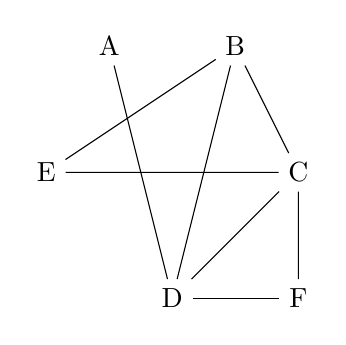
\begin{tikzpicture}[scale=.8]
      \node (A) at (2,4) {A};
      \node (B) at (4,4) {B};
      \node (C) at (5,2) {C};
      \node (D) at (3,0) {D};
      \node (E) at (1,2) {E};
      \node (F) at (5,0) {F};

      \foreach \from/\to in {A/D,B/C,B/D,B/E,C/D,C/E,C/F,D/F}
        \draw (\from) -- (\to);
    \end{tikzpicture}

  \item Zestaw kolorów:
    \begin{tikzpicture}[scale=.8]
      \node [0] (A) at (0,0) {};
      \node [1] (B) at (0.5,0) {};
      \node [2] (C) at (1,0) {};
      \node [3] (D) at (1.5,0) {};
      \node [4] (E) at (2,0) {};
      \node [5] (F) at (2.5,0) {};
    \end{tikzpicture}

  \item Przykładowy wynik:

    \begin{tikzpicture}[scale=.8]
      \node [0] (A) at (2,4) {A};
      \node [0] (B) at (4,4) {B};
      \node [1] (C) at (5,2) {C};
      \node [2] (D) at (3,0) {D};
      \node [2] (E) at (1,2) {E};
      \node [0] (F) at (5,0) {F};

      \foreach \from/\to in {A/D,B/C,B/D,B/E,C/D,C/E,C/F,D/F}
        \draw (\from) -- (\to);
    \end{tikzpicture}
\end{itemize}



\subsubsection{Krok 0}

\begin{itemize}
  \item Graf:

    \begin{tikzpicture}[scale=.8]
      \node [3] (A) at (2,4) {A};
      \node [4] (B) at (4,4) {B};
      \node [0] (C) at (5,2) {C};
      \node [3] (D) at (3,0) {D};
      \node [4] (E) at (1,2) {E};
      \node [0] (F) at (5,0) {F};

      \foreach \from/\to in {A/D,B/C,B/D,B/E,C/D,C/E,C/F,D/F}
        \draw (\from) -- (\to);
    \end{tikzpicture}

  \item Lista tabu: pusta
\end{itemize}


\subsubsection{Krok 1}

\begin{itemize}
  \item Akcja:
   \begin{tikzpicture}[->,scale=.8]
     \node [4] (1) at (0,0) {E};
     \node [3] (2) at (1.5,0) {E};

     \foreach \from/\to in {1/2}
       \draw (\from) -> (\to);
   \end{tikzpicture}

  \item Wartość funkcji celu: $-4$

  \item Graf:

    \begin{tikzpicture}[scale=.8]
      \node [3] (A) at (2,4) {A};
      \node [4] (B) at (4,4) {B};
      \node [0] (C) at (5,2) {C};
      \node [3] (D) at (3,0) {D};
      \node [3] (E) at (1,2) {E};
      \node [0] (F) at (5,0) {F};

      \foreach \from/\to in {A/D,B/C,B/D,B/E,C/D,C/E,C/F,D/F}
        \draw (\from) -- (\to);
    \end{tikzpicture}

  \item Lista tabu:
    \begin{tikzpicture}[scale=.8]
      \node [4] (E) at (0,0) {E};
    \end{tikzpicture}
\end{itemize}



\subsubsection{Krok 2}

\begin{itemize}
  \item Akcja:
   \begin{tikzpicture}[->,scale=.8]
     \node [3] (1) at (0,0) {A};
     \node [0] (2) at (1.5,0) {A};

     \foreach \from/\to in {1/2}
       \draw (\from) -> (\to);
   \end{tikzpicture}

  \item Wartość funkcji celu: $-8$

  \item Graf:

    \begin{tikzpicture}[scale=.8]
      \node [0] (A) at (2,4) {A};
      \node [4] (B) at (4,4) {B};
      \node [0] (C) at (5,2) {C};
      \node [3] (D) at (3,0) {D};
      \node [3] (E) at (1,2) {E};
      \node [0] (F) at (5,0) {F};

      \foreach \from/\to in {A/D,B/C,B/D,B/E,C/D,C/E,C/F,D/F}
        \draw (\from) -- (\to);
    \end{tikzpicture}

  \item Lista tabu:
    \begin{tikzpicture}[scale=.8]
      \node [3] (A) at (-1,0) {A};
      \node [4] (E) at (0,0) {E};
    \end{tikzpicture}
\end{itemize}



\subsubsection{Krok 3}

\begin{itemize}
  \item Akcja:
   \begin{tikzpicture}[->,scale=.8]
     \node [0] (1) at (0,0) {F};
     \node [4] (2) at (1.5,0) {F};

     \foreach \from/\to in {1/2}
       \draw (\from) -> (\to);
   \end{tikzpicture}

  \item Wartość funkcji celu: $-12$

  \item Graf:

    \begin{tikzpicture}[scale=.8]
      \node [0] (A) at (2,4) {A};
      \node [4] (B) at (4,4) {B};
      \node [0] (C) at (5,2) {C};
      \node [3] (D) at (3,0) {D};
      \node [3] (E) at (1,2) {E};
      \node [4] (F) at (5,0) {F};

      \foreach \from/\to in {A/D,B/C,B/D,B/E,C/D,C/E,C/F,D/F}
        \draw (\from) -- (\to);
    \end{tikzpicture}

  \item Lista tabu:
    \begin{tikzpicture}[scale=.8]
      \node [0] (F) at (-2,0) {F};
      \node [3] (A) at (-1,0) {A};
      \node [4] (E) at (0,0) {E};
    \end{tikzpicture}
\end{itemize}



\subsubsection{Krok 4}

\begin{itemize}
  \item Akcja:
   \begin{tikzpicture}[->,scale=.8]
     \node [0] (1) at (0,0) {A};
     \node [4] (2) at (1.5,0) {A};

     \foreach \from/\to in {1/2}
       \draw (\from) -> (\to);
   \end{tikzpicture}

  \item Wartość funkcji celu: $-14$

  \item Graf:

    \begin{tikzpicture}[scale=.8]
      \node [4] (A) at (2,4) {A};
      \node [4] (B) at (4,4) {B};
      \node [0] (C) at (5,2) {C};
      \node [3] (D) at (3,0) {D};
      \node [3] (E) at (1,2) {E};
      \node [4] (F) at (5,0) {F};

      \foreach \from/\to in {A/D,B/C,B/D,B/E,C/D,C/E,C/F,D/F}
        \draw (\from) -- (\to);
    \end{tikzpicture}

  \item Lista tabu:
    \begin{tikzpicture}[scale=.8]
      \node [0] (A) at (-2,0) {A};
      \node [0] (F) at (-1,0) {F};
      \node [3] (A) at (0,0) {A};
    \end{tikzpicture}
\end{itemize}



\subsubsection{Krok 5}

\begin{itemize}
  \item Akcja:
   \begin{tikzpicture}[->,scale=.8]
     \node [0] (1) at (0,0) {C};
     \node [5] (2) at (1.5,0) {C};

     \foreach \from/\to in {1/2}
       \draw (\from) -> (\to);
   \end{tikzpicture}

  \item Wartość funkcji celu: $-14$

  \item Graf:

    \begin{tikzpicture}[scale=.8]
      \node [4] (A) at (2,4) {A};
      \node [4] (B) at (4,4) {B};
      \node [5] (C) at (5,2) {C};
      \node [3] (D) at (3,0) {D};
      \node [3] (E) at (1,2) {E};
      \node [4] (F) at (5,0) {F};

      \foreach \from/\to in {A/D,B/C,B/D,B/E,C/D,C/E,C/F,D/F}
        \draw (\from) -- (\to);
    \end{tikzpicture}

  \item Lista tabu:
    \begin{tikzpicture}[scale=.8]
      \node [0] (C) at (-2,0) {C};
      \node [0] (A) at (-1,0) {A};
      \node [0] (F) at (0,0) {F};
    \end{tikzpicture}
\end{itemize}
\section{Projekty testów}
Przetestowane zostaną następujące aspekty programu:

\subsection{Poprawność działania}
Poprawność działania programu zostanie zweryfikowana przy pomocy testów jednostkowych.

\subsection{Wydajność}
\begin{itemize}
 \item Wydajność algorytmu zostanie zmierzona z użyciem zestawu grafów testowych różniących się liczbą wierzchołków i krawędzi.
 \item Dla celów testowych program zostanie zmodyfikowany tak, aby jako dane wejściowe przyjmował wstępnie pokolorowany graf.
  Pozwoli to:
  \begin{itemize}
   \item pominąć etap przygotowania grafu (patrz pkt. \ref{sec:exmpl_graph_prep}), a tym samym osiągnąć deterministyczne działanie programu,
   \item zbadać wpływ wstępnego pokolorowania na wydajność algorytmu.
  \end{itemize}
 \item Uzyskane wyniki zostaną ujęte w sprawozdaniu końcowym.
\end{itemize}


\end{document}
